\section{Extended Objective Sensitivities}
\label{sec:objective_supplement}
\subsection{Exploratory Scalarization}
We evaluate $J_\alpha(S)=\alpha C(S)/|R_{\mathrm{wf}}|+(1-\alpha)H(S)$ at seven weights, $\alpha\in\{0,0.10,0.25,0.50,0.75,0.90,1\}$. These greedy solutions trace an observed tradeoff curve. Neither the finite weight sweep nor the approximation guarantee establishes the global Pareto frontier or a universally preferred weight.

% Auto-generated Pareto Frontier Table for Q1 Journal Expansion
\begin{table*}[t]
\centering
\small
\caption{Multi-objective Pareto frontier across scalarization weight $\alpha$ at budget $|S|=100$ ($|R_{\text{wf}}| = 7{,}171$).}
\label{tab:q1_pareto_frontier}
\begin{tabular}{lrrrrrrrr}
\toprule
& \multicolumn{4}{c}{Package-Projected Graph} & \multicolumn{4}{c}{Version-Continuous Graph}\\
\cmidrule(lr){2-5} \cmidrule(lr){6-9}
Scalarization $\alpha$ & $C$ & $C$ (\%) & $H$ (\%) & $P$ & $C$ & $C$ (\%) & $H$ (\%) & $P$\\
\midrule
0.00 (Exact Union) & 4,407 & 61.46\% & 33.79\% & 534 & 4,479 & 62.46\% & 40.59\% & 527\\
0.10 & 4,591 & 64.02\% & 33.65\% & 530 & 4,714 & 65.74\% & 40.37\% & 553\\
0.25 & 4,809 & 67.06\% & 32.98\% & 604 & 4,855 & 67.70\% & 39.94\% & 634\\
0.50 (Balanced Sweet Spot) & 5,020 & 70.00\% & 31.19\% & 626 & 5,000 & 69.73\% & 38.65\% & 648\\
0.75 & 5,403 & 75.35\% & 21.69\% & 779 & 5,239 & 73.06\% & 31.75\% & 695\\
0.90 & 5,529 & 77.10\% & 14.15\% & 794 & 5,509 & 76.82\% & 14.97\% & 826\\
1.00 (Greedy Coverage) & 5,538 & 77.23\% & 11.48\% & 800 & 5,516 & 76.92\% & 13.10\% & 817\\
\bottomrule
\end{tabular}
\end{table*}


\begin{figure}[t]
\centering
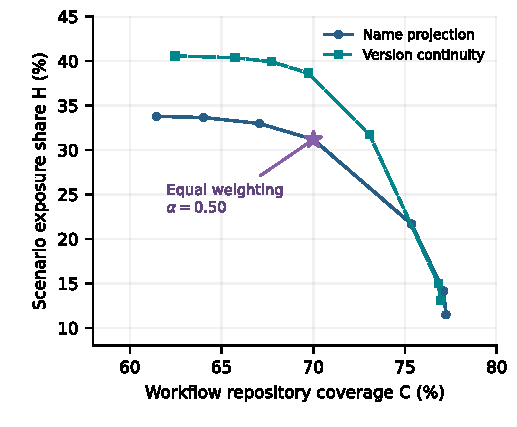
\includegraphics[width=\columnwidth]{q1_pareto_frontier.pdf}
\caption{Observed greedy scalarization results at budget 100. Connecting seven evaluated settings guides the eye; the curve is not a certified global Pareto frontier. Equal weighting is a sensitivity choice.}
\label{fig:q1_pareto_frontier}
\end{figure}

At $\alpha=0.50$, the name graph gives $C=5{,}020$, $H=31.19\%$, and $P=626$; the version graph gives $C=5{,}000$, $H=38.65\%$, and $P=648$. The name result retains 90.65\% of greedy's baseline coverage and 92.31\% of exact union's H. Relative to greedy, it loses 518 covered repositories and gains 19.71 percentage points of H. Relative to exact union, it gains 613 repositories and loses 2.60 points of H. A preferred operating point requires review costs and stakeholder preferences that were not measured here.

\subsection{Strict Zero-Anchored Threshold Sensitivity}
\label{sec:quorum_exclusion}

Multi-token incidents motivate asking how many unhardened source identities remain, but token count is not a measured release quorum. In LiteLLM's final account, credentials served different roles, including deletion of records after publication~\cite{litellm2026}. We evaluate the explicit strict rule in Eq.~\ref{eq:strict_quorum}, retaining only the 7,158 endpoints with observed sources and excluding all 13 source-free endpoints:
\begin{equation}
P_k(S)=\left|\left\{r\in R_+:t_r(S)=0\ \lor\ (n_r\ge k\ \land\ t_r(S)<k)\right\}\right|.
\end{equation}
The unguarded condition $t_r(S)<k$ credits every endpoint with $n_r<k$ even at zero hardening. In the strict model, a single-source endpoint must have its sole maintainer hardened at every threshold, and any endpoint with $n_r<k$ requires complete exclusion. This ensures a zero baseline for each tested $k$; it is not equivalent to subtracting the old zero-budget count.

A protection interpretation still requires a measured policy in which every successful attack needs the designated number of distinct upstream identities with no bypass. Our graph lacks package-level signer groups, role constraints, and bypass privileges. Two unrelated single-maintainer dependencies can each poison a consumer even if their combined source cardinality is two. Table~\ref{tab:q1_quorum_exclusion} is therefore a structural sensitivity analysis, not a count of empirically protected repositories.

% Auto-generated Generalized k-of-n Quorum Exclusion Table for Q1 Journal Expansion
\begin{table*}[t]
\centering
\small
\caption{Residual-source threshold counts $P_k(S)$ and coverage across maintainer hardening strategies ($|R_{\text{wf}}| = 7{,}171$).}
\label{tab:q1_quorum_exclusion}
\begin{tabular}{lrrrrrrrr}
\toprule
Prioritization Strategy & Budget & $C(S)$ & $C$ (\%) & $H(S)$ (\%) & $P_1(S)$ & $P_2(S)$ & $P_3(S)$ & $P_5(S)$ \\
 & $|S|$ & & & & ($k=1$) & ($k=2$) & ($k=3$) & ($k=5$) \\
\midrule
Portfolio Size                 & 10 & 3,435 & 47.90\% & 1.59\% & 391 & 1,915 & 2,433 & 3,093 \\
                               & 25 & 4,067 & 56.71\% & 4.38\% & 430 & 1,974 & 2,563 & 3,194 \\
                               & 50 & 4,446 & 62.00\% & 6.14\% & 503 & 2,025 & 2,613 & 3,244 \\
                               & 100 & 4,579 & 63.85\% & 7.96\% & 577 & 2,065 & 2,669 & 3,281 \\
\midrule
Greedy Coverage                & 10 & 4,331 & 60.40\% & 3.79\% & 351 & 1,846 & 2,406 & 3,080 \\
                               & 25 & 4,854 & 67.69\% & 6.08\% & 514 & 1,976 & 2,487 & 3,176 \\
                               & 50 & 5,196 & 72.46\% & 8.73\% & 638 & 2,039 & 2,552 & 3,232 \\
                               & 100 & 5,538 & 77.23\% & 11.48\% & 800 & 2,112 & 2,602 & 3,268 \\
\midrule
Exact Union                    & 10 & 3,910 & 54.53\% & 4.48\% & 343 & 1,825 & 2,385 & 3,105 \\
                               & 25 & 4,284 & 59.74\% & 9.86\% & 427 & 1,995 & 2,596 & 3,244 \\
                               & 50 & 4,321 & 60.26\% & 18.09\% & 441 & 2,011 & 2,609 & 3,324 \\
                               & 100 & 4,407 & 61.46\% & 33.79\% & 534 & 2,137 & 2,760 & 3,523 \\
\midrule
Pareto Hybrid ($\alpha=0.50$)  & 10 & 4,331 & 60.40\% & 3.79\% & 351 & 1,846 & 2,406 & 3,080 \\
                               & 25 & 4,795 & 66.87\% & 7.68\% & 498 & 1,948 & 2,505 & 3,194 \\
                               & 50 & 5,001 & 69.74\% & 14.96\% & 605 & 2,102 & 2,689 & 3,390 \\
                               & 100 & 5,020 & 70.00\% & 31.19\% & 626 & 2,153 & 2,719 & 3,415 \\
\midrule
Direct Supermodular $P(S)$     & 10 & 3,976 & 55.45\% & 2.58\% & 479 & 1,856 & 2,392 & 3,070 \\
                               & 25 & 4,239 & 59.11\% & 4.15\% & 618 & 1,880 & 2,424 & 3,124 \\
                               & 50 & 4,604 & 64.20\% & 6.55\% & 803 & 1,983 & 2,517 & 3,177 \\
                               & 100 & 5,020 & 70.00\% & 13.23\% & 1,022 & 2,074 & 2,636 & 3,337 \\
\bottomrule
\end{tabular}
\end{table*}


At budget 100, Pareto Hybrid has $P_1=626$, $P_2=961$, $P_3=1{,}018$, $P_5=1{,}063$. Greedy Coverage has $P_1=800$, $P_2=1{,}145$, $P_3=1{,}125$, $P_5=1{,}105$. Exact Union has $P_1=534$, $P_2=793$, $P_3=901$, $P_5=1{,}022$. Direct $P$ has $P_1=1{,}022$, $P_2=1{,}169$, $P_3=1{,}286$, $P_5=1{,}383$. The source-cardinality distribution is $n_r=0$: 13; $n_r=1$: 1,716; $n_r=2$: 546; $n_r=3$: 354; $n_r=4$: 347; and $n_r\ge5$: 4,195. All strict zero-budget counts are zero.

The same ordered maintainer selections are reused at all thresholds, and the Direct $P$ strategy continues to optimize its original $k=1$ heuristic. Counts are nondecreasing with nested hardening budgets for a fixed $k$. Comparisons across $k$ represent different hypothetical policies and need not be monotone, because endpoints with $n_r<k$ revert to complete-exclusion requirements.

For an additional hypothetical sensitivity, uniform control efficacy $\eta$ gives $H_\eta(S)=\eta H(S)$. At $\eta=0.90$, Pareto Hybrid yields $28.07\%$ effective scenario exposure reduction. This uniform multiplier preserves all $H$ rankings and does not estimate a real bypass rate, correlate account failures, or model CI compromise. Its values are assumptions, not incident-derived estimates.

\subsection{Heterogeneous Weight Sensitivities}
% Generated by scripts/reconcile_full_manuscript.py
\begin{table*}[t]
\centering
\footnotesize
\caption{Budget-100 outcomes under assumed weights. Each H column has its own stipulated denominator; weights are not estimated compromise probabilities.}
\label{tab:q1_heterogeneous_weights}
\begin{tabular}{lrrrrrr}
\toprule
Selection & C & H (\%) & Account-sole (\%) & Log (\%) & Package-sole (\%) & P\\
\midrule
Exact union & 4,407 & 33.79 & 77.30 & 40.15 & 27.32 & 534\\
Greedy coverage & 5,538 & 11.48 & 74.19 & 18.52 & 23.40 & 800\\
Portfolio & 4,579 & 7.96 & 70.26 & 15.06 & 13.72 & 577\\
Hybrid (0.50) & 5,020 & 31.19 & 80.41 & 38.93 & 28.51 & 626\\
Account-sole aware & 4,919 & 22.59 & 88.04 & 33.09 & 44.53 & 707\\
Log-portfolio aware & 4,603 & 31.91 & 81.42 & 42.91 & 33.17 & 514\\
Package-sole aware & 4,718 & 19.39 & 80.03 & 23.61 & 67.37 & 642\\
\bottomrule
\end{tabular}
\end{table*}


The account-sole weight increases an account's contribution according to its number of sole-maintained packages; it does not restrict its reachable endpoints to those packages. Ranking by that weighted reach captures 88.04\% of the stipulated account-sole mass. This is concentration under an assumed weighting, not nine-tenths of measured ecosystem risk.

The separate package-sole quantity unions reach only from each account's sole-maintained packages. Under that definition, unweighted greedy captures 23.40\%, unweighted exact union 27.32\%, and package-sole-aware ranking 67.37\%. The latter gain is 40.05 percentage points relative to unweighted exact union. Its uniform coverage is 4,718 repositories and $P=642$. These results distinguish account weighting from package-restricted reach. A single observed maintainer is not evidence about review quality or an empirically fitted probability of compromise.
